\chapter{Submersions, immersions and embeddings}

\section{Basic definitions}

\begin{definition*}
    Let \(F:M\to N\) be smooth. The \dhighlight{rank} of \(F\) at \(p\in M\)
    is the rank of the linear map \(dF_p:T_p M \to T_{F(p)}M\).
\end{definition*}

Smooth maps, which have full rank (highest possible rank, i.e. \(\text{rank} F=\max(m,n)\)) are particularly important:
\begin{definition*}
    Let \(F:M^m\to N^n\) be smooth. \marginnote{\(M^m,N^n\) means \(M,N\) are \(m,n\) dimensional manifolds}
    We say \begin{itemize}
        \item \(F\) is a \dhighlight{submersion} if \(dF_p\) is surjective, for all \(p\in M\) (\(m\geq n\))
        \item \(F\) is an \dhighlight{immersion} if \(dF_p\) is injective, for all \(p\in M\) (\(m\leq n\))
    \end{itemize}
\end{definition*}

\begin{lemma}\label{lem:4.1}
    Given \((m,n)\in \N_+\times \N_+\), let \(\Mat(m\times n)\equiv \R^{m\times n}\).
    The subset \(\Mat(m\times n)^{\text{full rank}}\coloneqq \{A\in \Mat(m\times n)\mid A\text{ has full rank}\}\)
    is open in \(\Mat(m\times n)\).
\end{lemma}

\begin{proof}
    Fix \(M\in\Mat(m\times n)^{\text{full rank}}\). Without loss of generality \(m\leq n\), otherwise 
    apply \(\Mat(m\times n)\to \Mat(n\times m),A\mapsto A^T\). By definition 
    there exists a submatrix \(M'\), obtained by deleting \(n-m\) columns, which is invertible.
    Now the map \marginnote{\(M\) is fixed and \(F\) depends on \(M\), but it does not matter here!}
    \begin{align*}
        \Mat(m\times n)\stackrel{F:M\mapsto M'}{\to} \Mat(m\times m)\stackrel{\text{det}(\cdot)}{\to} \R
    \end{align*}
    is continuous, since booth the forgetful \(F\) and det is smooth.
     \[M\in (\det\circ F)^{-1}(\underbrace{\R\setminus\{0\}}_{\text{open}})\subset \Mat(m\times n)^{\text{full rank}}\]
    since \(M\) was arbitrary this completes the proof.
    \begin{figure}[H]
        \centering
        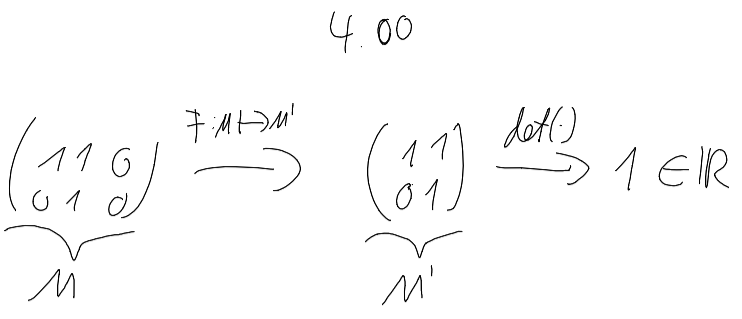
\includegraphics[width=.7\textwidth]{sketch_04_00.png}
        \caption{Sketch 4.00}
    \end{figure}
\end{proof}

\begin{lemma}\label{lem:4.2}\marginnote{The property of full rank is stable under small pertubation!}
    Fix \(F:M^m\to N^n,p\in M\).
    \begin{enumerate}
        \item If \(dF_p\) is injective, then there exists a neighborhood of \(p\) on which 
              \(dF_{\cdot}\) is injective. 
        \item If \(dF_p\) is surjective, then there exists a neighborhood of \(p\) on which 
        \(dF_{\cdot}\) is surjective. 
    \end{enumerate}
\end{lemma}

\begin{proof}
    This is a local statement. We can therefore assume that \(M,N\) are open subsets of \(\R^m,\R^n\) respectively.
    Then \[dF_{(\cdot)}:M\to \Mat(n\times m)\] 
    is smooth, hence continuous. By assumption \(dF_p\in \Mat(n\times m)^{\text{full rank}}\). But \(\Mat(n\times m)^{\text{full rank}}\), so 
    the preimage is open (by lemma \ref{lem:4.1}) and contains \(p\).
\end{proof}

\begin{remark}\marginnote{important: contains both a definition and a counterexample!}
    \begin{enumerate} % TOFIX
        \item If \(F:M\to N\) is both an immersion and a submersion, then we say that \(F\) is a \dhighlight{local diffeomorphism}. We will see (Rank theorem %TOFIX
        ) that \(F\) is a local diffeomorphism \(\iff\forall p\in M\exists p\in U: F\restrict{U}\) is a diffeomorphism.
        \item be warned. local diffeomorphism need not be global: \begin{alignat*}{10}
            \R^2&\equiv \C\supset& S^1=&\{|z|=1\}\to &S^1\\
            (x,y)&\mapsto x+iy &z&\xmapsto{\phantom{\{|z|=1\}\to}}  &z^2
        \end{alignat*}
    \end{enumerate}
\end{remark}

\begin{definition*}
    An immersion is an \dhighlight{embedding} if it is a homeomorphism onto its image 
    with the subspace topology.
\end{definition*}

\begin{example}
    \begin{figure}[H]
        \centering
        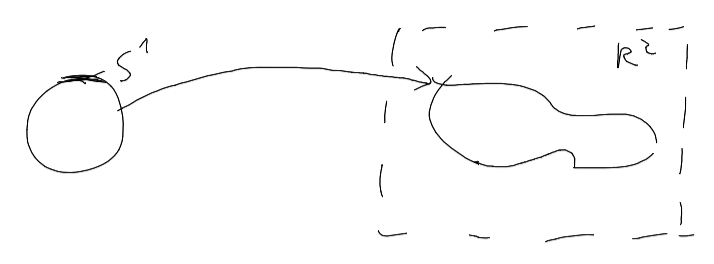
\includegraphics[width=.7\textwidth]{sketch_4_01.png}
        \caption{Sketch 4.01}
    \end{figure}
    Another example: \[S^n=\{(x_0,\dots,x_n)\in\R^{1+n}\mid\sum x_i^2=1\}\subset\R^{1+n}\]
    with \[i:S^n\hookrightarrow \R^{1+n}\]

    \dhighlight{Non-examples}
    \begin{figure}[H]
        \centering
        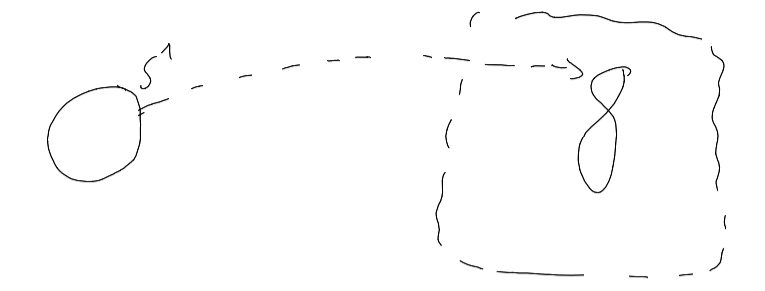
\includegraphics[width=.7\textwidth]{sketch_4_02.png}
        \caption{Sketch 4.02}
    \end{figure}
    parametrized by \[t\mapsto (\sin t,\sin 2t)\]
    and 
    \begin{align*}
        \R&\mapsto \R^2/\Z^2&=S^1\times S^1\\
        t&\mapsto (t,\alpha t) & \alpha \in\R\setminus \Q 
    \end{align*}
    Can show\footnote{not obvious, non-examable} that the image is dense. It is an immersion, but no a homeomorphism!
\end{example}








